\documentclass[pdftex,twocolumn,10pt,letterpaper]{article}
\usepackage{graphicx, times}
\usepackage{wrapfig}
\graphicspath{{.}}

\setlength{\textheight}{9.0in}
\setlength{\columnsep}{0.25in}
\setlength{\textwidth}{6.50in}
\setlength{\topmargin}{0.0in}
\setlength{\headheight}{0.0in}
\setlength{\headsep}{0.0in}

\begin{document}

\title{ Review of Stream Processing System }
\author{
    Shawn Zhong, Suyan Qu, Sulong Zhou \\
    \{wzhong36, squ27, szhou78\}@wisc.edu\\
    Group No. 7
}
\date{October 17, 2019}

\interfootnotelinepenalty=10000

\maketitle

\section{Introduction}

The explosion of modern information and computer science technology systems has extremely accelerated the development of data science. The ubiquitous social network, e-commerce platform and search engine continuously produce steady flows of high-volume data. Meanwhile, handling and analyzing real-time big data have become core demands for business and industry. This dramatic escalation in volumes of stream data is challenging existing data processing systems because of high-volume of users, low-latency of processing, heterogeneous resources and burstiness of events.  

In order to deal with the emerged challenges from 3 major perspectives(volume, velocity and variety) of stream data, and satisfy the needs of related markets, many stream data processing platforms targeted in scalability, fault tolerance and computing speed have been developed and deployed, such as Twitter’s Heron~\cite{Kulkarni:2015:THS:2723372.2742788}, LinkedIn’s Samza~\cite{Noghabi:2017:SSS:3137765.3137770} and Apache Flink~\cite{Carbone2015ApacheFS}. Meanwhile, a lot of efforts have been put into how to evaluate the performance of these frameworks when dealing with stream data. 

Theoretically and practically, benchmark rises in response to evaluate the performance of these frameworks. Considering the fast speed of the invention and development of the stream data processing systems, a set of universal standards is required to provide accurate, comprehensive, and uniformed measurement across diversity of stream data processing frameworks. 

In this work, we propose a review for current efficient standards for 5 different stream data processing frameworks. The standards are not only based on technique workflow and metrics, such as task scheduling, resource utilization, data processing model, fault toleration, scalability, throughput and latency, but also social parameters, such as community engagement and user inclusion.


% \section{Related Work}



\section{Background}

\subsection{Stream Processing}
Big data computing models are mainly divided into batch computing, stream computing, interactive computing, graph computing, etc. Among them, stream computing and batch computing are two main big data computation modes, which are applicable to different big data application scenarios. 

Stream data (or data stream) refers to [a series of dynamic data that comes indefinitely (source needed!!!) ]. The value of data decreases with time, so it must be calculated in real time to give a response in seconds. 

Streaming processing, as its name implies, is the processing of data streams, which is a real-time calculation. Batch calculation is a method of uniformly collecting data, storing it in a database, and then performing batch processing on the data. 

The difference is mainly reflected in the following aspects: 

\begin{enumerate}
\item Data timeliness: stream computing requires real-time, low latency, whereas batch computing can tolerate high latency. 

\item Data characteristics: stream data is generally dynamic, there is no boundary, and the batch data is generally static data. 

\item Application scenarios: Streaming computing applications are used in real-time scenarios, where timeliness requirements are relatively high, such as real-time recommendation, business monitoring, etc. Batch computing generally says batch processing, applications in real-time requirements are not high, offline computing scenarios, data analysis, offline reports, and more. 

\item Execution method: The task of stream computing is continuous, and the task of batch computing is completed in one time.
\end{enumerate}

\subsection{Stream Processing Systems}

\subsubsection{Apache Storm\cite{toshniwal2014storm}}
Apache Storm is Twitter's first generation of real-time fault-tolerant stream data processing system. In Storm, tasks are handled on a master node called Nimbus. It communicates with a set of Zookeepers that monitors the supervisors of a set of worker nodes. Storm does not have any data structure for storage. Data storage is handled by external data management systems such as Hadoop File System. 

\subsubsection{Apache Heron}
Heron is the second-generation real-time stream data processing system used in Twitter improved from Apache Storm. In Storm, each worker runs multiple threads for different jobs, leading to no resource isolation between different jobs. Heron improves by replacing Nimbus by an external scheduler such as Aurora, which can provide more resource isolation. In addition, in Heron, scheduler no longer communicates with Zookeepers for workers' heartbeats and task assignments. Instead, it communicates with Topology Masters for task assignment, while a separate monitoring system will manage the server status, resource usage, and other related metrics for failure recovery and performance improvement. 

\subsubsection{Spark Streaming}

Spark Streaming is an extension of the Spark core API that enables high-throughput, fault-tolerant real-time streaming data processing. In Spark Streaming, Master is mainly responsible for overall cluster resource management and application scheduling; Worker is responsible for resource management of a single node (startup of drivers and executors, etc); Driver is the place where the user entry program is executed, which includes DAG generation, stage division, task generation, and scheduling; Executor are responsible for executing tasks, feedback execution status and execution results.

\subsubsection{Apache Flink}

Apache Flink is a distributed processing engine for streaming data and batch data. The stream-first approach provides low latency, high throughput, per-item processing, and the ability to compute complex calculations. Flink integrates with all common cluster resource managers such as Hadoop YARN, Apache Mesos, and Kubernetes but can also be setup to run as a stand-alone cluster by resource-manager-specific deployment modes. Low latency is guaranteed by local state optimization in memory. Flink applications are parallelized in a distributed system. Therefore, an application can leverage virtually unlimited amounts of CPUs, main memory, disk and network IO. 

\subsubsection{Kafka Streams}
Kafka Streams is a real-time stream computing library that relies on existing Kafka clusters to provide distributed, highly fault-tolerant, real-time stream computation. Kafka Streams is designed to be lightweight. It has no external dependencies other than Kafka Stream Client library, ans can be easily embedded in Java applications. 

\section{Comparisons}

\subsection{Computation Model}

TODO: Introduction

In Apache Storm and Heron, the computation graph is called topology. After the user designing a topology, it is then submitted to the cluster, where the master node is responsible for allocating code to the worker nodes, and the worker nodes are responsible for executing the code. There are two roles in a topology: spout and bolt. Data is passed between spouts, which send data streams as  tuples, and bolts are responsible for converting data streams.

Spark Streaming is an extension of the core Spark API. Unlike Storm, it does not process a single stream of data at the same time. Instead, it splits the data stream by time interval before processing the data stream. The abstraction for continuous data streams in Spark Streaming is called DStream (Discretized Stream), which is a small batch of RDD (Elastic Distributed Dataset). RDD can be converted by any function and sliding data window for parallel operation.

\subsection{Scalibility}


Kafka Streams: 
However, it is difficult to meet the complex computing requirements of a large amount, and the input and output of the data are dependent on the Kafka cluster. For other data sources, Kafka connect is required to input the data into the Kafka, and then processed by the Kafka Streams program. Therefore, Kafka Streams is more suitable for scenarios where the computational complexity is small and the data flow process is from Kafka to Kafka.

\begin{figure*}[!ht]
    \centering
    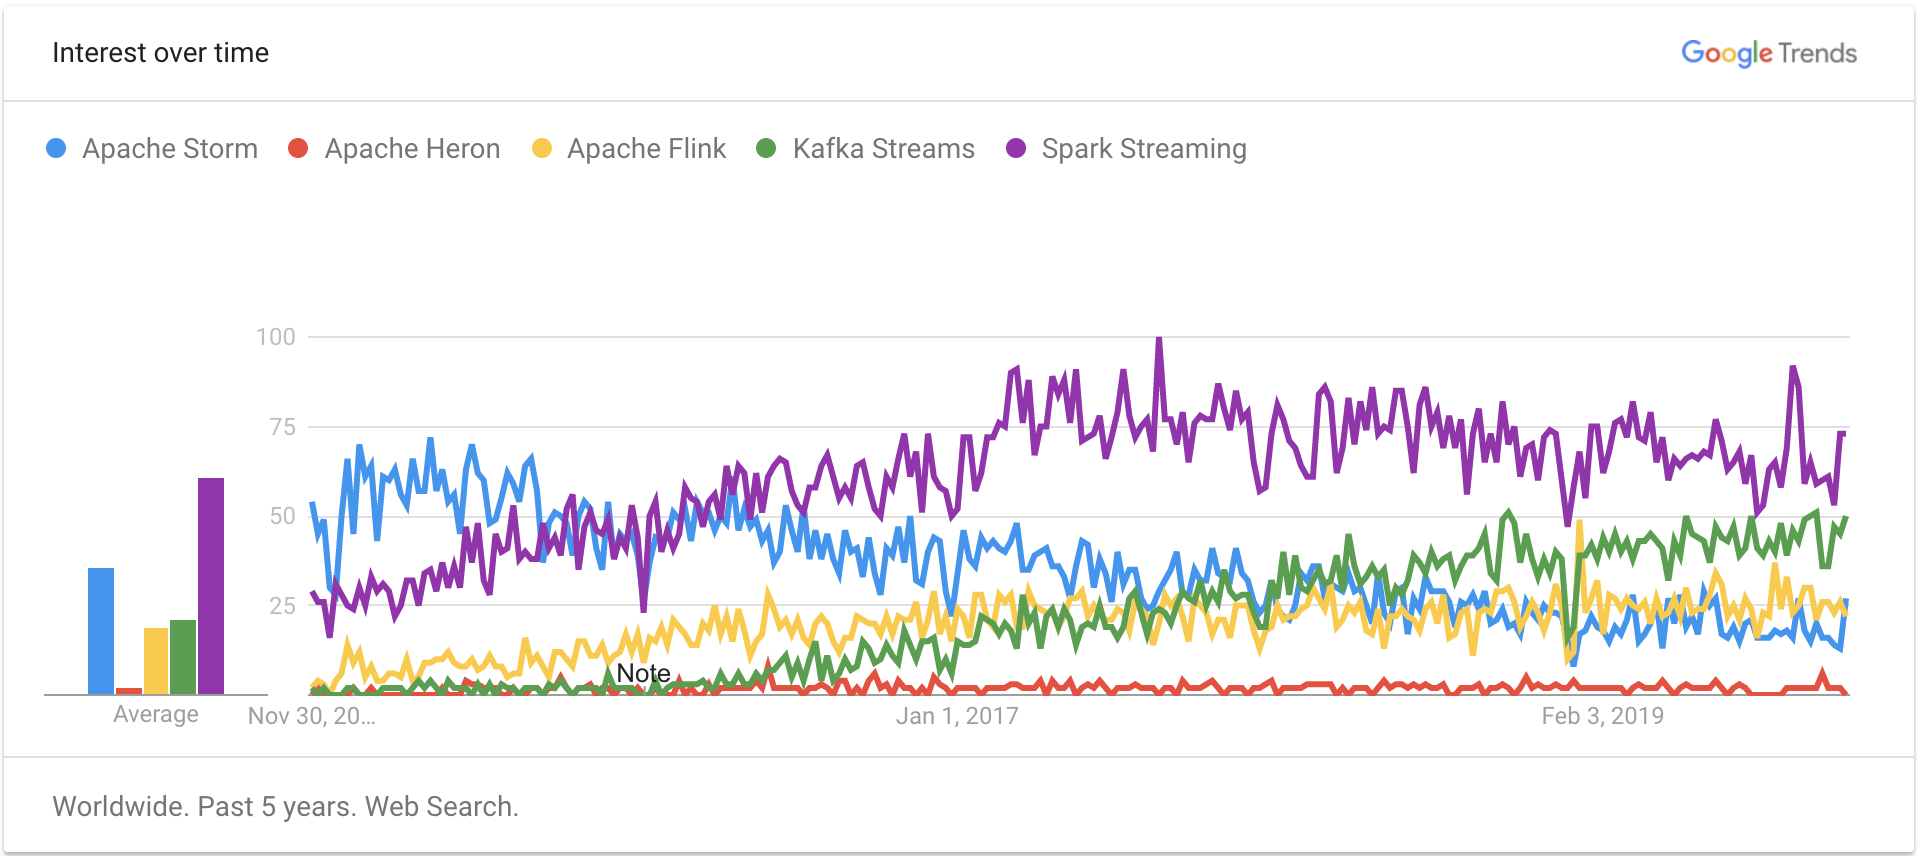
\includegraphics[width=\textwidth]{trend.png}
    \caption{Google search trends\cite{googletrend} for different stream processing systems over the past 5 years.}
    \label{fig:trend}
\end{figure*}

\subsection{Timeliness}

Heron is a real-time stream processing. Once the data comes, it is processed. 

Spark Streaming is micro-batch processing. After the data arrives, it will be processed for a while.

\subsection{Fault Tolerence}



\subsection{Social Factors}
In this section, we consider the social influences of different stream processing frameworks. 

Figure \ref{fig:trend} shows the Google search trend over the past 5 years. It is noticed that Apache Storm was the most popular stream processing system. However, Spark Streaming quickly exceeds Storm since it is easier to implement and deploy. Spark Streaming also provides cheaper fault tolerance and capability to seamlessly integrate with non-stream processing tasks, while only slightly increase latency. These characteristics makes it the most popular stream processing system over the past 3 years. On the other hand, we see a steady decreasing trend for Storm. In fact, Twitter is one of the companies that move away from using Storm to Heron in 2015. Yet Heron depends on a wide range of external tools such as Hadoop File System, Aurora, Zookeeper, etc, making it extremely complicated to deploy and implement in large scale. As a result, it remains the least popular system over the past 5 years. It is also worth noting that Apache Kafka is also experiencing a steady increase in popularity, with various companies such as Uber Technology Inc and Palo Alto Network Inc using it nowadays. 




% \begin{tabular}{ |c|c|c|c|c| } 
%  \hline
%                     & Heron & Spark Streaming & Flink  \\ 
%  \hline
%  Data flow model    & Real-time & Micro-batch &Real-time  \\ 
%  \hline
%  Latency            & Low & High & Low \\ 
%  \hline
% \end{tabular}


\section{Benchmark}

\subsection{System setup}

We deploy the stream processing system to a Kubernetes cluster of 5 nodes on Google Cloud Platform. The machine types for each node is n1-standard-4, which has 4 vCPU, 15 GB memory, and 100 GB SSD. 

\section{Conclusions}

{
\bibliographystyle{ieeetr}
\bibliography{ref}
}
\end{document}
